\important{Artificial Intelligence Library (May 19, 2024)}
\label{Artificial-Intelligence-Library}
\chapterauthor{Ian Smith}
\info{Ian Smith}{Artificial Intelligence Library}{May 19, 2024}
\subsection*{Abstract}

Within Vex VRC, the programmers on VRC team 7686X attempt to use reinforcement machine learning to conquer traditionally skillful and challenging tasks. They navigate, explain, and use the complex landscape of bleeding-edge artificial intelligence commonly found in fully autonomous road vehicles. Although not discussing anything not currently known in the field of reinforcement learning, the paper attempts to give the reader a from-the-ground-up understanding of reinforcement learning. Follow the authors on their 8-month journey of learning machine learning; all while attempting to document it along the way.

\subsection*{Concept of Machine Learning}

While not a novel concept, machine learning and artificial intelligence have gained significant traction in recent years. Fundamentally, Machine Learning involves utilizing computational algorithms to perform actions, learn from the outcomes, explore variations, and optimize results iteratively. This core idea of optimization through trial and error manifests in various forms, such as decision-making, predictive analytics from datasets, and developing advanced mathematical models to solve complex problems.

\subsubsection*{Types of Machine Learning}
Machine Learning can be broadly categorized into three types:
\begin{itemize}
    \item \textbf{Supervised Learning:} Algorithms learn from labeled datasets, making predictions based on input-output pairs.
    \item \textbf{Unsupervised Learning:} The model finds patterns in data without labeled responses.
    \item \textbf{Reinforcement Learning:} An agent learns by interacting with an environment, and receiving rewards or penalties for its actions.we
\end{itemize}
In the context of robotics, reinforcement learning is especially useful as it allows the robot to learn optimal actions through trial and error. "\cite{lex_friedman}"

This prompts a question: how can we leverage machine learning (ML) in Vex robotics? This application arises from the need for extremely precise control over robots in various scenarios, including matches, programming skills, and autonomous periods. Artificial intelligence could manage both adaptive strategies and robot control based on sensor and known environment data.

\subsection*{Q Learning vs. Deep Q Learning}
Q-learning is a reinforcement learning algorithm where an agent learns to choose actions that maximize cumulative rewards in a given environment. It stores a Q-table representing the expected utility of actions in specific states. However, this approach struggles with large state spaces. "\cite{sentdex_dqn}"

Deep Q-Learning addresses this by using a neural network to approximate the Q-values, enabling the agent to handle much more complex environments by generalizing from its experiences.

In robotic control, one of the most common methods of using Machine Learning is Deep Q Learning, also known as Deep Q Network (DQN). The concept of Deep Q Learning originates from Q Learning. In Q Learning, a table is generated for environmental observations, associating an output with each observed input "\cite{sentdex_dqn}." An example might resemble the following:

\begin{center}
    \begin{table}[!hbt]
        \centering
        \begin{tabular}{|c|c|c|c|c|}
             \hline
                & \(x_1\) & \(x_2\) & \(x_3\) & \(x_4\) \\ [0.5ex]
              \hline
              \(y_1\) & left & right & up & up\\
              \hline
              \(y_2\) & down & right & left & up \\
              \hline
              \(y_3\) & up & left & down & left\\ [1ex]
              \hline
        \end{tabular}
        \caption{Example Q Table}
        \label{tab:my_label}
    \end{table}
\end{center}

This representation is relatively straightforward to comprehend and computationally cost-effective to process. During training, the algorithm explores various solutions and selects the best one. In a simple simulation environment with few variables, this approach works effectively. However, in real-world applications, a Q-learning algorithm typically performs poorly due to unexpected variables. Thus, a more sophisticated solution is required: Neural Networks.

\subsection*{Neural Networks}

Neural Networks are based on the concept that any control logic can be represented by a mathematical equation or algorithm. So, how do we create a one-size-fits-all algorithm capable of finding any mathematical function? Computer scientists in the 1950s, namely Frank Roseblatt discovered that a complex network of \(y = mx + b\) equations can be tuned by a computer through an optimizer "\cite{3b1b_1}."

\begin{figure}[H]
    \centering
    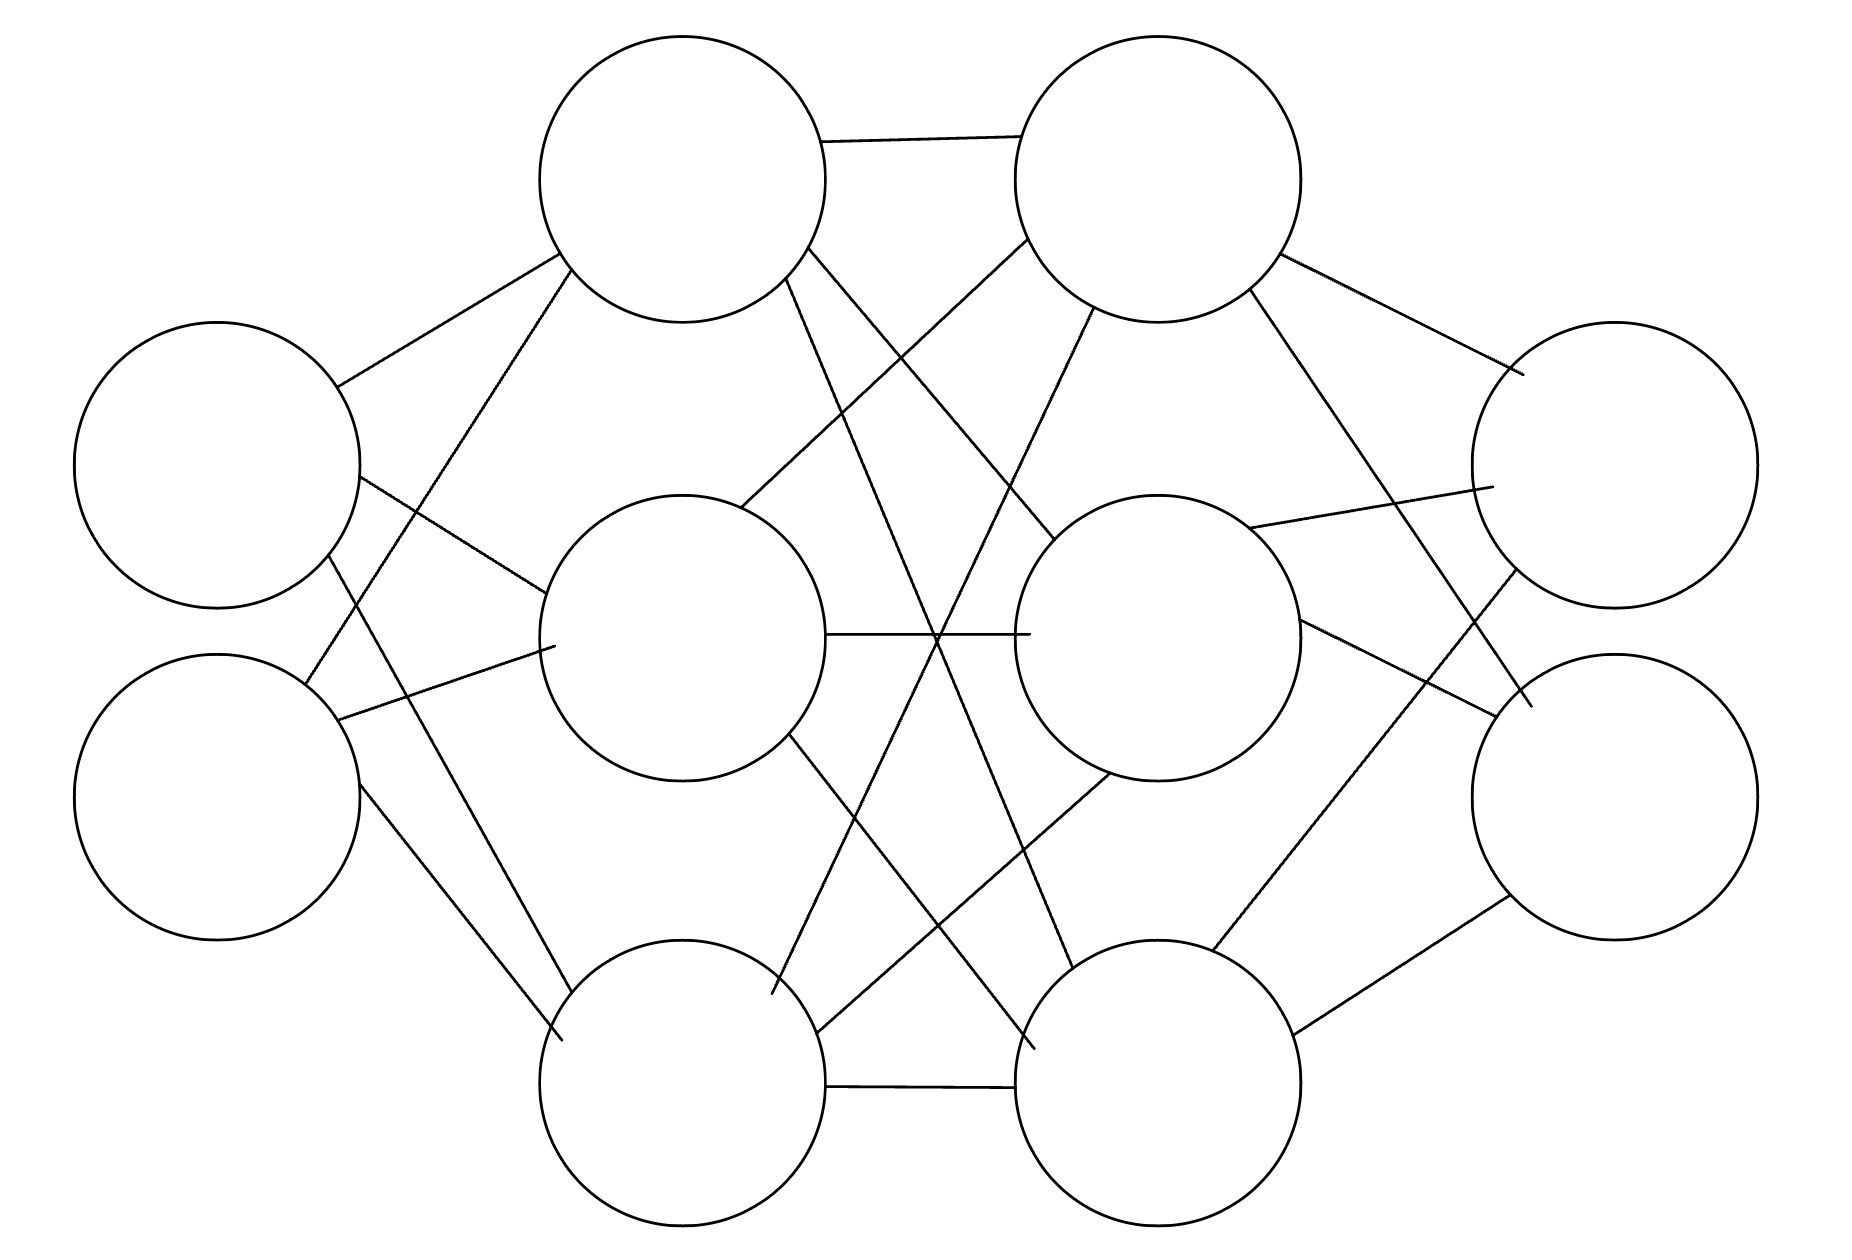
\includegraphics[width=0.7\linewidth]{images/NueralExample.jpg}
    \caption{Example of a Simple Neural Network}
    \label{Example of Simple Neural Network}
\end{figure}

Each dot represents a neuron, and each line represents a different \(y = mx + b\) connection. This model is a proven method for artificial intelligence, with almost all advanced intelligence systems using this layout. There are a few critical parts to note when examining a neural network. The first set of neurons is called the "Input Layer," and the last is called the "Output Layer." The actual complexity of a neural network lies within the "Hidden Layers," which are neither input nor output. Two related factors affect hidden layers: Layer Size and the Number of Layers. These two factors directly impact both the performance of the decision-making process and the computational expense of the intelligence. A very complex network will be more accurate but also more computationally expensive. This means that Neural Networks are a balance of performance and expense. The expense can be represented by this equation:

\[O(n^x)\]

Where: \(x\) = number of layers; \(n\) = neurons per layer

Despite the number of layers being exponential, it is still more efficient to use larger layers rather than more layers. With the neural network able to process data, all it needs is a method to train.

\subsection*{Training}

There are several methods for training neural networks. Common models include calculating how correct or incorrect a model was, otherwise known as a loss function, then performing a backward pass and calculating the gradient to train. This approach does not work well in our case because there is no objective way to determine right and wrong that is inherently obvious. For our scenario, where we want to train our network to find the best outcome, it is best to use a genetic algorithm to determine the best-performing model in each batch. After selecting the best model, after reproducing and slight manipulation, a new best can be determined. To do this, we can randomize each value of the Q Table slightly from the previous value. To control the amount of randomization, we can use a calculus principle known as epsilon ($\epsilon$). Epsilon signifies a small non-zero number approaching zero. It is also possible to use an exponential decay function to determine epsilon. With a way to control how extreme the tables will be, it is time to begin writing the code.

\section*{Creation of Neural Network Library}

Everything will be done in the programming language C++, as it is the most universal and widely accepted in Vex Robotics. Examples may appear in mathematics or pseudo code.

\subsection*{Linear Algebra}

To perform the fundamental operations of a neural network, some linear algebra is required to find the output of a neural layer. The chosen method involves a complex web of \(y = mx + b\) formulas. In the layer-by-layer linear algebra, \(x\) is represented by the common name "inputs," \(y\) by "weights," and \(b\) by "biases." This naming convention will be used for all provided math. The general form for calculations is the dot product of the transpose of weights added to biases "\cite{sentdex_nn}." For the following examples, let the inputs be:

\[
\begin{pmatrix} 
-1.0 & 3.1 \\
1.9 & -0.2 \\
4.0 & -2.1 \\
\end{pmatrix}
\]

weights be:

\[
\begin{pmatrix}
    -3.5 & 1.2 & 0.5\\
    4.1 & -3.5 & 7.1\\
\end{pmatrix}
\]

and biases be:

\[
\begin{pmatrix}
    0.7\\
    -1.2\\
    2.3\\
\end{pmatrix}
\]

\subsubsection*{Transpose}

To properly match the shapes of matrices, a transpose must be performed on weights before performing the dot product operation. This function reverses the x and y planes of a matrix. This can be represented as:

\[
\begin{pmatrix}
    -3.5 & 1.2 & 0.5\\
    4.1 & -3.5 & 7.1\\
\end{pmatrix}^\top
=
\begin{pmatrix}
    4.1 & -3.5\\
    -3.5 & 1.2\\
    7.1 & 0.5\\
\end{pmatrix}
\]

After performing the transpose of weights, the matrices are ready for the next step: dot product.

\subsubsection*{Dot Product}

The next process is finding the dot product, sometimes referred to as the cross product. This can be found with the following formula:

\[
c_{ij} = \sum_{k=1}^{n} a_{ik} \cdot b_{kj}
\]

Using this formula, we can apply it to our two matrices:

\[
\begin{pmatrix}
    -1.0 & 3.1 \\
    1.9 & -0.2 \\
    4.0 & -2.1 \\
\end{pmatrix}
\cdot
\begin{pmatrix}
    4.1 & -3.5\\
    -3.5 & 1.2\\
    7.1 & 0.5\\
\end{pmatrix}
=
\begin{pmatrix}
    -14.95 & 7.22\\
    8.49 & -6.89\\
    23.75 & -16.52\\
\end{pmatrix}
\]

\subsubsection*{Addition}

The final step in the linear algebra is addition, which is a relatively straightforward process:

\[
\begin{pmatrix}
    -14.95 & 7.22\\
    8.49 & -6.89\\
    23.75 & -16.52\\
\end{pmatrix}
+
\begin{pmatrix}
    0.7\\
    -1.2\\
    2.3\\
\end{pmatrix}
=
\begin{pmatrix}
    -14.25 & 7.92\\
    7.29 & -8.09\\
    26.05 & -14.22\\
\end{pmatrix}
\]

\subsection*{Forward Pass}

Now that the essential math behind the network is done, a forward pass can be performed to calculate the linear algebra dynamically based on inputs. When programming this, structs were used for the math with a function call for forward pass. When doing a forward pass, it is just a process of computing the whole network. To introduce non-linearity in the network, a Rectified Linear Unit (ReLU) is used. This can be mathematically expressed as:

If \(x > 0\):

\[
y = x
\]

Otherwise:

\[
y = 0
\]

This system works well for its designed task and is computationally inexpensive to run. The only issue is that the output layer cannot have the ReLU activation applied to introduce negative numbers in our case. Most algorithms have some kind of activation function at the end, but we will not need one in our scenario. However, other activation functions were still added to the namespace for use at user discretion.

\subsection*{Epsilon Greedy}

Epsilon (\(\epsilon\)) is a calculus principle that signifies a very small non-zero value. In our case, \(\epsilon\) is used in the greedy function that determines the cost of exploitation vs. exploration. Our Epsilon Greedy will be determined by an exponential decay function:

\[
\epsilon = e^{-m \cdot x} + b
\]

Where:

\(m\) = Learning Rate

\(x\) = Current Episode

\(y\) = Randomness

\(b\) = Minimum Learning Rate

This equation creates a decay function that finds a low non-zero value to determine how random the mutation to the previous data will be. When programming this, a random value was multiplied by the coefficient of randomness \(\epsilon\) and added to the previous value in the neuron.

\subsection*{File Management System}

Coincidentally, most of the time coding was spent trying to universally, efficiently, and effectively manage data related to neural networks. To do this successfully, all data will be formatted into ".txt" files in a manner that makes sense. To do this, the files have to be initialized with the desired dimensions, read, and then written to. Many algorithms went into the formatting of files.

\subsubsection*{Creation of Formatted .txt Files}

To process and transfer data quickly and easily within different systems, formatted files with ".txt" extensions will be used to store this data. The code that processes the build request creates a new file with the designated amount of neurons and layers to fit dimensions correctly. A second function "write()" writes a 5-dimensional array into the file.

\subsubsection*{Reading Formatted .txt Files}

The "read()" function reads a formatted ".txt" file and commits it to a 5-dimensional array for processing. After a file is read, it can either be mutated through the mutation process and then run, or put directly into the "run()" function for release versions.

\subsection*{Implementing Linear Algebraic Functions}

After an output has been calculated, it may be useful to run it through an activation function to format it into a useful response. This includes softmax activation, which puts the data through an exponential function; argmax activation, which places data on a spectrum (usually between [0, 1]) based on the highest and lowest outputs of the output layer; and ReLU, which is the same as the ReLU inside the algorithm, ignoring all values less than 0 "\cite{activation_functions_website}."

\subsection*{Infinite Training}

After all of the main functions were programmed such as forward passes, file I/O operations, and activation functions, the algorithm was fully capable of computing and training. The last key to making the algorithm work is implementing a way to infinitely train the neural network. A function was devised where the results could be passed along with the network that got the score. The best neural networks are returned based on the score given with the largest being the best run. When it is time to do the data writing, the best are selected based on the top returned and the specified amount to be returned. From that point the new mutated neural networks can be read and the process can be repeated in a conditional loop for training. 

\section*{Implementation and Changes}

After the AI was done being written, it was implemented in a few different test cases. Immediately, it was noted that the model would perform, by converging over time. It passed the linear regression test, but it proved to have difficulty with a more complex test. This more complex test was one where it had to control linear velocity in a 2D environment and score objects within a certain amount of time. This was a task that the AI failed, which caused some questions to arise about neural network optimization.

\subsection*{Code Changes for Optimization}

The first course of action was to change all C++ "float" values (32-bit floating point numbers), to the "double" or "long float" type (64-bit floating point numbers). This proved to help a little bit with the performance of the network due to the increased precision, yet, it wasn't enough.

\section*{Starting Over}

\subsection*{Introduction to Reinforced Learning}

Reinforced learning is a subdiscipline of machine learning where experience is used to update a loss function rather than a traditional loss function. Traditional loss functions might include mean squared error, and Deep Q Learning (as discussed in the last chapter) which might use loss as a Q function.

%add equations here (MSE, Bellman Equation)

\[MSE = \frac{1}{n}\sum_{i=1}^{n} (y_{i} - \hat{y_{i}})^{2}\]

Where $n$ is the predictions in the batch,

      $\hat{y}$ is the predicted output value (from the neural network),
      
      and $y$ is the actual known value.
"\cite{g4g_mse}"

\subsection*{Gradient Descent}

Gradient Descent is an optimization algorithm used to minimize the loss function in a neural network. It works by iteratively adjusting the model's parameters (weights) to reduce the difference between the predicted and actual outcomes. This is achieved by calculating the gradient, which indicates the direction and rate of change in the loss function.

When optimizing a neural network, a number must be formulated to update the weights of a neural network. But how do we get this number? More importantly, how can we optimize this number to achieve the desired effect?

Gradient descent is a method from multi-variable calculus that forms a multi-dimensional graph. Unfortunately, we do not have a way of seeing the graphed data directly. When looking at our data, our goal is to write a program that finds the "lowest $y$" value, where $y$ is the loss of the neural network. Unfortunately, for the sake of this paper at least, it is impossible to find the absolute minima, so, we will have to settle for a relative minima in this case. The concept of gradient descent can be best represented on a 2D plane "\cite{3b1b_2}."

\begin{figure}[H]
    \centering
    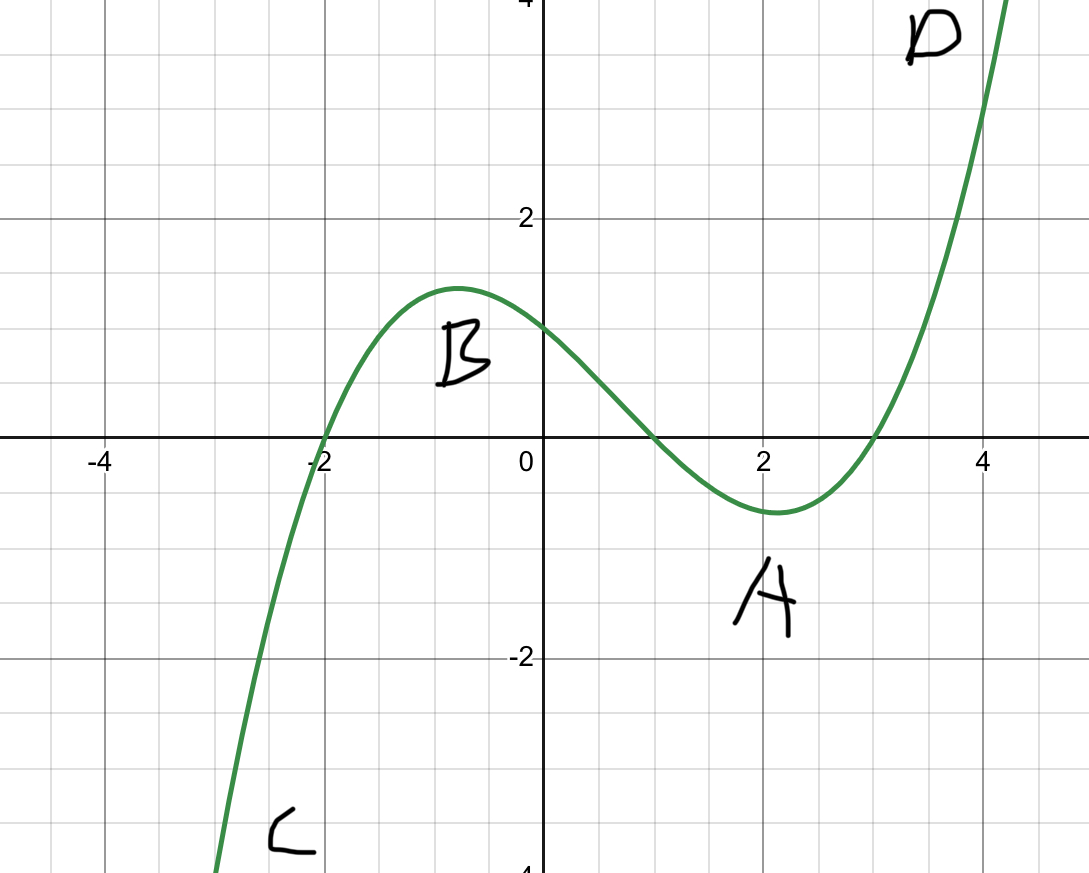
\includegraphics[width=0.75\textwidth]{images/GradientDescent.jpg}
    \caption{Visualization of Gradient Descent on a 2D Plane. Point A represents a local minimum, and Point C represents the global minimum.}
    \label{fig:gradient_descent}
\end{figure}

As shown in Figure \ref{fig:gradient_descent}, the algorithm starts at a point on the curve and takes steps proportional to the negative of the gradient at that point, eventually converging at the lowest point, or minimum, of the function.
In Figure \ref{fig:gradient_descent}, imagine starting at the point $(0, 1)$. From here, your goal is to reach the lowest point possible. For the example, let $A$ and $B$ respectively be local minima and maxima, and let $C$ and $D$ respectively be absolute minima and maxima for this example. From point $(0, 1)$ the reader needs a way to navigate to the lowest $y$ coordinate possible. The most popular method, and the one we will use, is to take a step and see what change that makes to the $y$ coordinate. Below in the table is each time step $t$, and the reward (in lowest y coordinate) $y$ or $r$. This can be represented by the following formula:

The general formula for updating the parameters using gradient descent is given by:
\[
\theta = \theta - \eta \cdot \nabla_\theta J(\theta)
\]
where:
\begin{itemize}
    \item $\theta$ represents the model parameters (weights).
    \item $\eta$ is the learning rate, which controls the size of the steps.
    \item $\nabla_\theta J(\theta)$ denotes the gradient of the loss function $J(\theta)$ with respect to the parameters.
\end{itemize}
"\cite{3b1b_2}"

\begin{center}
    \begin{table}[]
        \centering
        \begin{tabular}{|c|c|c|c|c|}
             \hline
              \(t\) & \((x, y)\) & \(r\) & \(\theta\) \\ [0.5ex]
              \hline
              \(0\) & $(0, 1)$ & $1$ & -\\
              \hline
              \(1\) & $(-0.5, 1.5)$ & $1.5$ & $+0.5$\\
              \hline
              \(2\) & $(0, 1)$ & $1$ & $-0.5$\\
              \hline
              \(3\) & $(0.5, 0.5)$ & $0.5$ & $-0.5$\\
              \hline
              \(4\) & $(1, 0)$ & $0$ & $-0.5$\\
              \hline
              \(5\) & $(1.5, -0.5)$ & $-0.5$ & $-0.5$\\
              \hline
              \(6\) & $(2, -0.7)$ & $-0.7$ & $-0.2$\\
              \hline
              \(7\) & $(2.5, -0.5)$ & $-0.5$ & $+0.2$\\
              \hline
              \(8\) & $(2, -0.7)$ & $-0.7$ & $-0.2$\\[1ex]
              \hline
        \end{tabular}
        \caption{Gradient descent Example}
        \label{tab:my_label}
    \end{table}
\end{center}

In Table \ref{tab:my_label}, we start at $(0, 1)$ with an initial reward of 1. At each time step $t$, change was calculated for the $y$ coordinate based on the gradient. The step size $\theta_t$ indicates whether the algorithm is moving towards a local minimum or maximum.

After establishing a basic understanding of gradient descent, let's look at a more relevant example. In this example, it showcases descending a complex 3D landscape. This might be what a simple neural network does when calculating its gradients throughout many episodes. When it reaches eventual local minima, that is seen as the point when training is complete.

\begin{figure}[H]
    \centering
    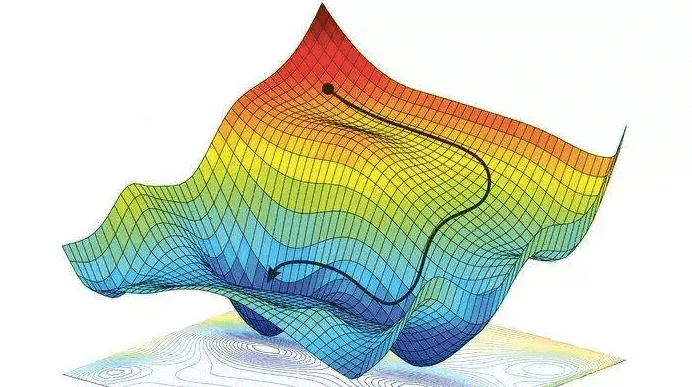
\includegraphics[width=0.75\linewidth]{images/IansColorGraph.png}
    \caption{3D Neural Network}
    \label{fig:3dneuralnetwork}
\end{figure}

This new change in direction yields the partial derivative ($\partial$) used in the next step for backpropagating through the neural network. From this point on in this book, $\partial$ will be used instead of $\theta$ to represent calculated gradients "\cite{3b1b_2}."

In neural networks, gradient descent is applied in the backpropagation process. The partial derivative $\frac{\partial J}{\partial \theta}$ represents how the loss changes with respect to each weight. By updating the weights using these gradients, we can minimize the overall loss and improve the network's predictions "\cite{3b1b_2}."

Note: \textit{The choice of learning rate $\eta$ is crucial; a value too large can cause the model to overshoot the minimum, while a value too small may result in slow convergence. Additionally, in complex, high-dimensional spaces, the algorithm may get trapped in local minima, making it difficult to find the absolute minimum.}

\subsection*{Backward Pass and Weight Update}

Once loss has been calculated using forward propagation, the next step is to update the neural network's weights to reduce this loss. This is achieved through the backward pass, a fundamental concept in training neural networks.

The backward pass is part of the backpropagation algorithm, which uses the chain rule of calculus to calculate the gradients of the loss function with respect to each weight in the network. These gradients tell the team how much each weight contributes to the loss, and they are used to update the weights in a way that minimizes the loss "\cite{3b1b_2}."

To understand this, imagine there is a simple neural network with one hidden layer. During forward propagation, we compute the output of each neuron, which is ultimately used to calculate the network's loss. Now, in the backward pass, we start from this loss and propagate backward through the network, layer by layer to calculate the gradients.

\subsubsection*{The Chain Rule and Gradient Calculation}

For each weight $w$ in the network, we need to find out how a small change in
$w$ affects the loss 
$L$. This is given by the gradient 
$\frac{\partial L}{\partial w}$
 . Using the chain rule, this gradient is calculated as:

\[\frac{\partial L}{\partial w} = \frac{\partial L}{\partial z} \cdot \frac{\partial z}{\partial w}\]
 
where $z$ is the input to the activation function of the neuron.

By taking the change in the loss function by the derivative of the activation function, we can multiply it by the input neuron, or as we solved for earlier as the output of a neuron with respect to weight.

By multiplying these two terms, we get the total gradient of the loss with respect to the weight 
$w$.

\subsubsection*{Weight Update Using Gradient Descent}

Once we have the gradient for each weight, the weights are updated using gradient descent. The algorithm for updating is:

\[w = w - \eta \cdot \frac{\partial L}{\partial w}\]
 
where $\eta$ is the learning rate, this equation adjusts the weight $w$ in the direction that reduces the loss. A positive gradient means the weight will decrease, while a negative gradient will increase.

\begin{center} \begin{table}[] \centering \begin{tabular}{|c|c|c|} \hline \textbf{Weight} & \textbf{Gradient} & \textbf{Updated Weight} 
\\ \hline $w_1$ & $0.1$ & $w_1 = w_1 - 0.01 \cdot (0.1)$
\\ \hline $w_2$ & $-0.3$ & $w_2 = w_2 - -0.01 \cdot (-0.3)$
\\ \hline $w_3$ & $0.05$ & $w_3 = w_3 - 0.01 \cdot (0.05)$
\\ \hline \end{tabular} \caption{Example of Weight Updates} \label{tab} \end{table} \end{center}

Table \ref{tab} shows how each weight is updated based on its gradient. The learning rate $\eta = 0.01$ controls the step size of the updates. When training, it is important to choose an appropriate learning rate; if it's too high, the network might not converge, and if it's too low, training can be very slow.

\subsubsection*{Backward Pass Further Explanation}

To visualize the backward pass, consider a neural network trained to classify images (convolutional neural network) "\cite{3b1b_1}." During the backward pass, the error is calculated at the output layer and then propagated backward through each layer. Each neuron's weight is adjusted based on how much it contributed to the final error. This process is repeated for each training input in the dataset until the network's weights converge to values that minimize the overall error.

Overall, the backward pass and weight update allow a reinforcement learning algorithm to learn from its mistakes by adjusting the weights in a way that reduces the error in future outputs according to the loss function.

\subsubsection*{Challenges and Solutions}

One challenge in the backward pass is the issue of vanishing or exploding gradients "\cite{he2015delvingdeeprectifierssurpassing}." When gradients become too small or too large, the network can either stop learning or become unstable due to large adjustments. Techniques like gradient clipping and proper initialization can help reduce gradient-related problems

In this section, we have covered how the backward pass and weight update are essential for training neural networks. With this foundation, we can now move on to more advanced optimization techniques that further refine the training process.

\subsection*{Gradient Momentum and Optimization}

In training neural networks, one of the primary goals is to accelerate convergence towards local minima while avoiding erratic updates and oscillations in the loss that can impede training progress. A widely used technique to achieve this is gradient momentum. By incorporating momentum, we can increase the efficiency and stability of the gradient descent algorithm by forcing lower minima "\cite{loshchilov2019decoupledweightdecayregularization}."

\subsubsection*{Understanding Momentum within Optimization}

Momentum in the context of gradient descent is similar to the concept of momentum in physics. In physics, momentum helps a moving object maintain its velocity despite resistance. Similarly, in optimization, momentum helps our weight updates move through the loss landscape more smoothly, reducing the oscillations in loss and thus gradients, enabling more efficient convergence.

Consider the standard gradient descent update rule from the last section:

\[w = w - \eta \cdot \frac{\partial L}{\partial w}\]
"\cite{loshchilov2019decoupledweightdecayregularization}"

This equation updates the weight $w$ directly based on the current gradient $\frac{\partial L}{\partial w}$. Although this strategy works, it can be sensitive to noisy gradients (or "sharp" changes in gradient), especially in complex loss landscapes. This sensitivity can cause the weight updates to oscillate, particularly when the gradient direction changes sharply between updates.

To address this, we introduce a momentum term, $v$, which is the exponentially weighted average of the past gradients. The momentum-based update rule is defined as follows:

\[v = \beta \cdot v_{t-1} + (1 - \beta) \cdot \frac{\partial L}{\partial w}\]

\[w = w - \eta \cdot v\]

In this formula: $\beta$ is the momentum coefficient, typically set at 0.99 in our case. $v$ accumulates the gradients over time, incorporating a fraction $\beta$ of the previous momentum $v_{t-1}$. $t$ indicates the current step of gradient calculation that the algorithm is in.
This update policy effectively smooths the gradient by incorporating historical gradients, reducing erratic change, and promoting more consistent steps towards the minima.

\subsubsection*{Visualizing Momentum}

To visualize the effect of momentum, imagine a ball rolling down a hilly terrain towards the lowest point. Without momentum, the ball will quickly change direction in response to small inclines or bumps, leading to a jagged path. With momentum, however, the ball can maintain its direction despite minor variations in the terrain, allowing it to glide more smoothly and reach the lowest point faster. Thus, think of $\beta$ in essence as a variable to control the weight of the ball "\cite{3b1b_2}."

\subsubsection*{Combining Momentum with Advanced Optimizers}

While momentum itself provides significant improvements over standard gradient descent, it can be further enhanced when combined with advanced optimizers such as Adam. Adam, or Adaptive Moment Estimation, incorporates momentum for both the first moment (mean $m$) and the second moment (uncentered variance $v$) of the gradients. The update rules for Adam are given by:

\[m_t = \beta_1 \cdot m_{t-1} + (1 - \beta_1) \cdot \frac{\partial L}{\partial w}\]

\[v_t = \beta_2 \cdot v_{t-1} + (1 - \beta_2) \cdot (\frac{\partial L}{\partial w})^2\]

\[\hat{m} = \frac{m_t}{1 - \beta^{t}_{1}}\] \[\hat{v}_t = \frac{v_t}{1 - \beta^{t}_{2}}\]

\[w = w - \eta \cdot \frac{\hat{m}_t}{\sqrt{\hat{v}_t} + \epsilon}\]

Here: $m_t$ and $v_t$ are the first and second-moment estimates, respectively. $\beta_1$ and $\beta_2$ control the exponential decay rates for these estimates, typically set to 0.9 and 0.999. $\epsilon$ is a small constant to prevent division by zero.
Adam's use of both momenta leads to a robust and adaptive optimizer that adjusts the learning rate for each parameter individually, resulting in a faster and more stable convergence "\cite{haarnoja2019learningwalkdeepreinforcement}."

\subsubsection*{Psuedo Code Example}

\begin{center} 
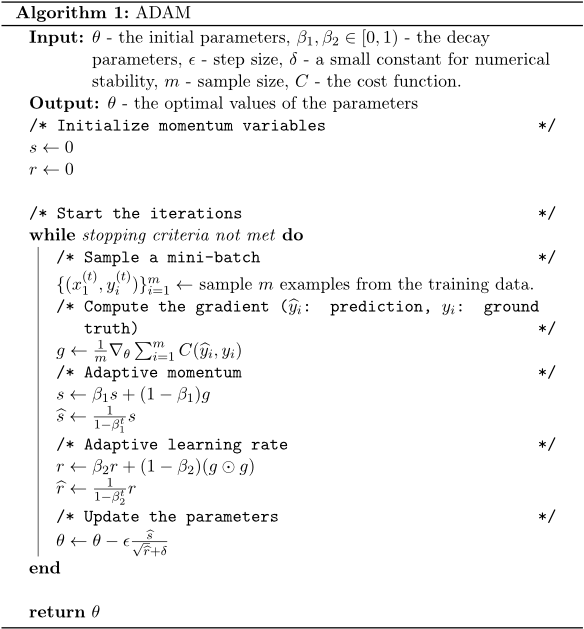
\includegraphics[width=0.75\textwidth]{images/ADAM.png} 
\label{fig}
\end{center}
"\cite{haarnoja2019learningwalkdeepreinforcement}"

\subsubsection*{Practical Considerations}

When implementing momentum in a neural network, there are several practical considerations:

Choosing the Momentum Coefficient $\beta$: Setting $\beta$ too high can cause the optimizer to overshoot the minima while setting it too low might diminish the benefits of momentum. A typical choice is 0.9, which balances stability and speed.

Learning Rate Adjustment: With momentum, the effective learning rate is increased. This means that the base learning rate $\eta$ might need to be reduced compared to standard gradient descent to prevent overshooting.

Gradient Clipping: When dealing with complex models, gradient clipping can be used alongside momentum to prevent large gradients from destabilizing the training process.

\subsubsection*{Conclusion}

Gradient momentum is a powerful technique that accelerates convergence and improves the stability of the training process. By incorporating past gradients, momentum helps smooth out the optimization path and overcome local minima more effectively. When combined with advanced optimizers like Adam, it provides a robust framework for training deep neural networks efficiently.

With an understanding of gradient momentum, we can further explore more sophisticated optimization techniques and strategies to enhance the training process of our neural network models.

\subsection*{Actor-Critic Learning (A2C)}

Actor-critic methods combine the benefits of both policy-based and value-based approaches in reinforcement learning, helping overcome some of the limitations of each. The main idea is to simultaneously train two components of the model: the Actor, which is responsible for selecting actions, and the Critic, which evaluates how good those actions are by calculating a value function. This complementary system allows for more efficient learning in complex environments.

\subsubsection*{Overview of Actor and Critic Components}

The \textbf{Actor} is a policy network that directly maps states to actions. It represents the agent's policy, determining what action should be taken in each state. Its role is to maximize the expected reward by producing actions that lead the agent toward more optimal states. During training, the Actor continuously adjusts its policy based on feedback from the Critic, refining its ability to select actions "\cite{openai_a2c}."

The \textbf{Critic}, on the other hand, evaluates the actions taken by the Actor. It estimates the value of the current state (or state-action pairs) and provides feedback to the Actor on how good the chosen actions are. This value estimate is crucial because it guides the Actor toward decisions that are expected to yield higher rewards over time. By estimating the future rewards more accurately, the Critic plays a pivotal role in stabilizing the learning process "\cite{openai_a2c}."

\subsubsection*{Advantage Function in A2C}

A2C improves upon traditional Actor-Critic methods by introducing an \textbf{Advantage Function}, which is used to calculate how much better (or worse) a specific action performed compared to the average. This refinement helps in mitigating variance in policy gradients, making the learning process more stable and efficient.

The advantage at time step $t$, denoted as $A(s_t, a_t)$, is given by:
\[A(s_t, a_t) = Q(s_t, a_t) - V(s_t)\]
Where $Q(s_t, a_t)$ is the state-action value function (estimating the total future reward if action $a_t$ is taken in state $s_t$), and $V(s_t)$ is the value function (estimating the expected reward from state $s_t$). By using this advantage, A2C trains the Actor-network more effectively by pushing it to favor actions that perform better than average, thus optimizing the policy over time.

\subsubsection*{Training Process}

The training process in A2C is an interplay between the Actor and Critic networks, with both learning concurrently. The Critic learns by minimizing the \textbf{Temporal Difference (TD) Error}:
\[TD_t = r_t + \lambda V(s_{t+1})-V(s_t)\]
Where $r_t$ is the reward at time step $t$, and $\gamma$ is the discount factor, which controls the emphasis on future rewards. The Critic uses this error to update the value function.

The Actor, in contrast, updates its policy using the policy gradient method. The key update rule for the Actor’s parameters $\theta$ is:
\[\nabla_\theta J(\theta) = E [\nabla_\theta \log \pi_\theta (a_t | s_t)A(s_t , a_t)]\]
This equation shows that the policy is adjusted in the direction that maximizes the advantage, thus leading to more optimal decision-making over time.

\subsubsection*{Benefits and Applications of A2C}

A2C has several advantages over traditional reinforcement learning algorithms. First, it reduces the variance in policy gradients by using the value function to stabilize updates, which can result in faster convergence. Secondly, by using a Critic, the method can incorporate more information from the environment, improving sample efficiency. Lastly, because the Actor and Critic are learned in parallel, A2C achieves a balance between exploration and exploitation, leading to better long-term results in complex environments.

In practice, A2C is commonly used in tasks where continuous action spaces or complex decision-making are required, such as robotic control or autonomous vehicular navigation, such as our case and inspiration. Its stability and ability to handle high-dimensional environments make it a powerful tool for solving challenging reinforcement learning problems.

\subsubsection*{Challenges and Extensions}

Despite its strengths, A2C can still suffer from high variance and instability in more complex environments. For this reason, extensions like \textbf{Advantage Actor-Critic (A3C)} and \textbf{Proximal Policy Optimization (PPO)} have been developed to further stabilize and optimize the learning process.

By addressing these challenges, A2C remains an integral part of modern reinforcement learning techniques, providing a strong foundation for more advanced and stable methods.

\subsection*{He Initialization and Gradient Clipping}

When training deep neural networks, managing how weights are initialized and how gradients are controlled during backpropagation are crucial for ensuring the model's convergence and stability. Two essential techniques that address these challenges are \textbf{He Initialization} and \textbf{Gradient Clipping}. Both methods play a pivotal role in maintaining smooth training dynamics, preventing common pitfalls such as vanishing or exploding gradients.

\subsubsection*{He Initialization}

Weight initialization is a critical step in setting up a neural network. If weights are poorly initialized, the model can either fail to learn or converge too slowly. \textbf{He Initialization}, named after Kaiming He, was introduced to address the issues of training deep networks, particularly for networks using ReLU (Rectified Linear Unit) or its variants as activation functions "\cite{he2015delvingdeeprectifierssurpassing}."

The key idea behind He Initialization is to preserve the variance of the weights throughout the network, allowing for efficient gradient flow during backpropagation. It achieves this by drawing weights from a distribution that takes into account the size of the previous layer, helping prevent the vanishing gradient problem that occurs in deeper networks. The formula for He Initialization is:

\[W = N(0, \frac{2}{n_{\text{in}}})\]

Where:

$W$ is the weight matrix for the current layer.
$n_{\text{in}}$ is the number of input units to the layer.
The variance is scaled by $\frac{2}{n_{\text{in}}}$, which adjusts the weight distribution based on the layer size.
By initializing weights in this manner, the network avoids the risk of saturating neurons, which can hinder learning, especially in the early stages of training. The network is able to maintain appropriate activation distributions throughout its layers, promoting faster and more stable convergence.

\subsubsection*{Why He Initialization Matters}

Consider the propagation of gradients in a deep neural network. As the gradient signal passes through many layers, its magnitude can diminish (vanishing gradients) or grow uncontrollably (exploding gradients). Both scenarios make it difficult for the network to learn. He Initialization counteracts these effects by ensuring that, at initialization, the variance of activations and gradients is neither too small nor too large.

This initialization method is particularly effective when paired with ReLU activations. ReLU's ability to sparsely activate neurons (by zeroing out negative values) works synergistically with He Initialization, allowing the network to learn efficiently while avoiding the pitfalls of poor weight scaling.

\subsubsection*{Gradient Clipping}

While proper initialization helps with stabilizing the network’s learning process, during training, gradients can still become unstable—particularly when they grow too large, a problem known as the \textbf{exploding gradient problem}. To address this, we use a technique called \textbf{Gradient Clipping}.

Gradient Clipping limits the magnitude of gradients to a specified threshold. By capping gradients at a maximum value, we prevent excessively large updates that could cause the model to diverge. The basic idea is simple: when the gradients exceed a predefined threshold, we scale them down, ensuring that they stay within a manageable range "\cite{zhang2020gradientclippingacceleratestraining}."

Mathematically, the update rule with Gradient Clipping for a gradient vector $\nabla_{\theta} L$ becomes:

\[\nabla_{\theta} L \leftarrow \frac{\nabla_{\theta} L}{\max (1, \frac{\|\nabla_{\theta} L\|}{\tau})}\]
 
Where:

$\nabla_{\theta} L$ is the gradient of the loss function $L$ with respect to the model parameters $\theta$.
$\tau$ is the threshold value for clipping.
If the magnitude of the gradient exceeds $\tau$, it is scaled down; otherwise, it remains unchanged. By limiting the gradient's size, we ensure that learning steps are not too aggressive, leading to a more stable training process.

\subsubsection*{Combining He Initialization and Gradient Clipping}

When used together, \textbf{He Initialization} and \textbf{Gradient Clipping} form a robust strategy for training deep neural networks. He Initialization lays the foundation for smoother and more stable weight updates, while Gradient Clipping provides a safety mechanism against runaway gradients that could otherwise destabilize the network.

The combination of these techniques is particularly useful in deep reinforcement learning environments, where the feedback signals (rewards) can be noisy or sparse. In these settings, managing gradient flow becomes critical to ensuring the model continues learning efficiently.

\subsection*{ADAMW Optimizer}

The \textbf{ADAMW optimizer} is a refinement of the widely-used ADAM optimizer, designed to address a specific shortcoming in how weight decay (regularization) is applied during the optimization process. It combines the power of adaptive learning rates and momentum, while correctly decoupling weight decay from the optimization step, leading to improved performance and generalization in deep neural networks.

\subsubsection*{Why ADAMW over ADAM?}

The traditional ADAM optimizer is known for its ability to handle noisy gradients and for adapting learning rates individually for each parameter. This makes ADAM an excellent choice for training deep models, especially when dealing with sparse or noisy data. However, ADAM applies $L_2$ regularization in a way that can interfere with the optimization process. The issue arises because ADAM incorrectly applies weight decay ($L_2$ regularization) to the gradient update itself, rather than the weights directly. This can distort the learning dynamics, especially in large-scale neural networks "\cite{loshchilov2019decoupledweightdecayregularization}."

The ADAMW optimizer resolves this by decoupling the weight decay from the gradient-based parameter updates. This allows weight decay to function solely as a mechanism for regularization, independent of the actual optimization step. The result is more effective regularization, leading to better generalization without slowing down the convergence rate.

\subsubsection*{How ADAMW Works}

To understand how ADAMW operates, it’s helpful to briefly revisit the standard ADAM optimizer. ADAM computes adaptive learning rates for each parameter by keeping track of two moving averages:

The first moment (mean) of the gradients, which is a form of momentum.
The second moment (uncentered variance) of the gradients, adjusts the learning rate based on the magnitude of the gradients.
The update rule for ADAM looks like this:

\[\theta_{t+1} = \theta_t - \eta \cdot \frac{\hat{m}_t}{\sqrt{\hat{v}_t} + \epsilon}\]
 
Where:

$\theta_t$ represents the model parameters at time step $t$.
$\eta$ is the learning rate.
$\hat{m}_t$ and $\hat{v}_t$ are bias-corrected estimates of the first and second moments, respectively.
$\epsilon$ is a small constant to prevent division by zero.
In ADAM, weight decay is incorrectly integrated into the gradient calculation. ADAMW, however, updates the weight decay independently of the gradient steps, as shown in the following update rule:

\[\theta_{t+1} = \theta_t - \eta \cdot (\frac{\hat{m}_t}{\sqrt{\hat{v}_t} + \epsilon} + \lambda \cdot \theta_t)\]

Where:

$\lambda$ is the weight decay factor, applied directly to the parameters $\theta_t$ rather than the gradient.
This subtle change ensures that the weight decay is applied correctly as a regularization technique, preventing overfitting while allowing the optimizer to take full advantage of its adaptive learning rate and momentum benefits.

\begin{center}
    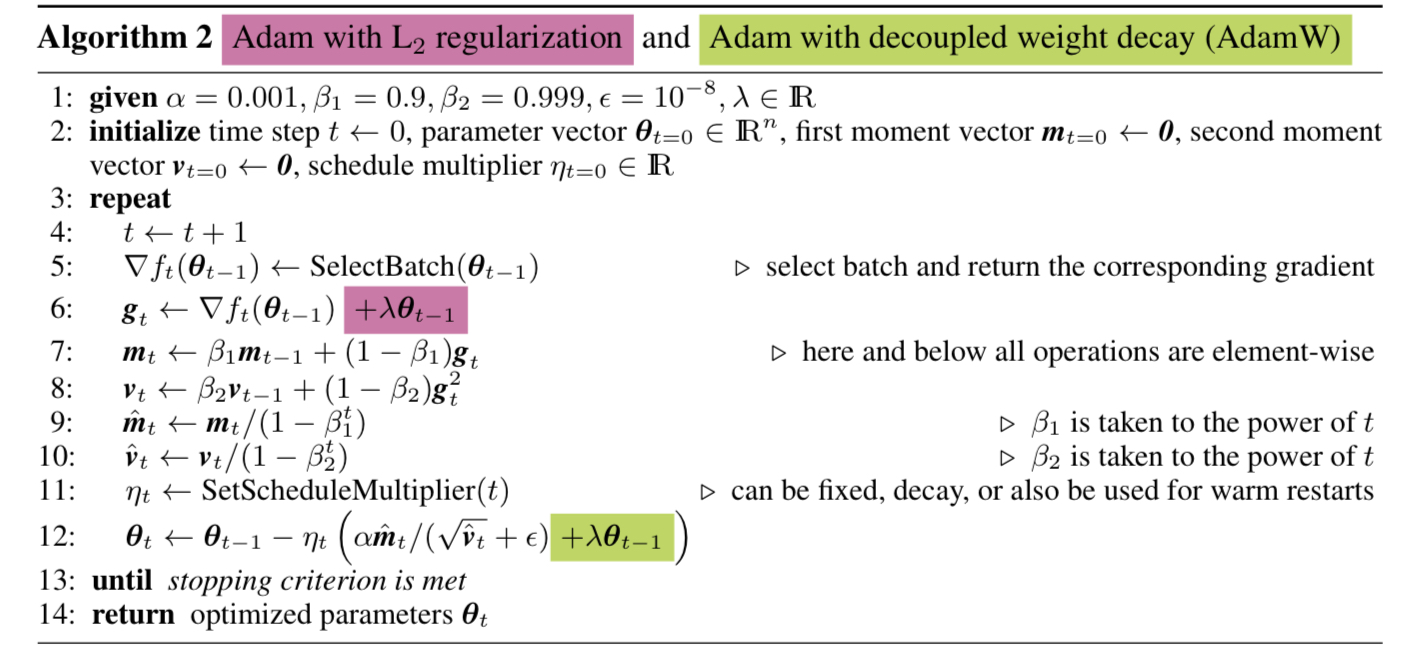
\includegraphics[width=0.75\textwidth]{images/ADAML2.jpg}
    "\cite{loshchilov2019decoupledweightdecayregularization}"
    \label{fig}
\end{center}

\subsubsection*{Benefits of ADAMW}

The ADAMW optimizer offers several advantages over the traditional ADAM optimizer, particularly in terms of generalization and training stability:

\textbf{Improved Generalization}: By decoupling weight decay from the adaptive gradient updates, ADAMW applies regularization more effectively, resulting in better generalization to unseen data.
\textbf{Faster Convergence}: Since weight decay is handled independently, ADAMW retains the fast convergence properties of ADAM without the interference caused by improper weight decay application.
\textbf{Better Control Over Regularization}: With ADAMW, weight decay operates purely as a regularizer, offering more control over how much penalty is applied to large weights. This helps mitigate overfitting, especially in deep networks with many parameters like the ones we will build.

\subsubsection*{Practical Applications of ADAMW}

In practice, ADAMW is now a default choice in many deep learning libraries, given its improvements over the standard ADAM optimizer. It is especially beneficial in scenarios where weight decay plays a critical role in regularization:

\textbf{Reinforcement Learning}: In environments where data is sparse and noisy, ADAMW can be particularly effective by stabilizing training and ensuring that models converge quickly without overfitting. This is important because our environment and sensors will be ever-changing and extremely noisy "\cite{loshchilov2019decoupledweightdecayregularization}."

\subsubsection*{Final Thoughts}

The ADAMW optimizer stands as a critical advancement over the traditional ADAM optimizer by decoupling the weight decay from the gradient updates. This subtle but important improvement enables more effective regularization, faster convergence, and better generalization in deep learning models. As neural networks grow deeper and more complex, ADAMW remains a vital tool for keeping training stable and ensuring that the model performs well on unseen data. As covered in the paper "\cite{loshchilov2019decoupledweightdecayregularization}", ADAMWR is an improvement yet upon ADAMW. This is an option open to the team if our agents continue to struggle with noisy data. 

\subsection*{Soft Actor-Critic Learning (SAC)}

\textbf{Soft Actor-Critic (SAC)} is an advanced reinforcement learning algorithm that combines the strengths of both policy-based and value-based methods. As a variant of the popular actor-critic architecture, SAC introduces the concept of entropy regularization to balance exploration and exploitation more effectively. It is designed for continuous action spaces and seeks to maximize both the expected reward and the entropy of the policy, making it a powerful tool for solving complex, high-dimensional tasks.

\subsubsection*{Key Principles of SAC}

At its core, SAC builds on two key principles: the actor-critic framework and the maximization of policy entropy. These principles allow SAC to provide better exploration during training while maintaining stability and efficiency in learning.

\textbf{Actor-Critic Architecture:} Like traditional actor-critic methods, SAC employs two neural networks:

The \textbf{actor}, which represents the policy and is responsible for selecting actions based on the current state.
The \textbf{critic}, which estimates the value of a given state-action pair and helps the actor learn by providing feedback on the quality of the actions taken.
What differentiates SAC from other actor-critic algorithms is its emphasis on policy entropy.

\textbf{Entropy Regularization:} Entropy in reinforcement learning measures the randomness in the policy’s action distribution. By encouraging higher entropy, SAC promotes exploration by ensuring the policy does not become too deterministic early in training. This is particularly useful in environments with sparse rewards, where exploring a wide range of actions can lead to discovering better strategies.

The objective function for the actor in SAC is a combination of expected reward and policy entropy:

Where:

$\pi$ represents the policy.
$r(s_t, a_t)$ is the reward for taking action $a_t$ in state $s_t$.
$\mathcal{H}(\pi(\cdot|s_t))$ is the entropy of the policy, encouraging exploration.
$\alpha$ is the temperature parameter that controls the balance between maximizing reward and entropy.
\subsubsection*{How SAC Works}

SAC operates in a way that integrates continuous exploration with efficient learning. Let’s break down the major components of the algorithm.

\textbf{Policy Learning:} The actor-network outputs a stochastic policy, meaning it learns a probability distribution over possible actions rather than a single deterministic action. This allows the agent to continue exploring, even in later stages of training, by sampling actions from this distribution. Over time, the policy becomes more refined, yet still retains a level of randomness for effective exploration.

\textbf{Value Learning:} SAC employs not one but \textbf{two Q-value networks} to estimate the value of state-action pairs. This is done to mitigate the issue of overestimation in value functions, which can destabilize learning. During training, the minimum of the two Q-value estimates is used to update the policy, ensuring that the agent doesn’t overestimate the value of any action.

\textbf{Temperature Adjustment:} The temperature parameter $\alpha$ governs how much exploration is encouraged by controlling the weight of the entropy term in the objective function. SAC introduces an adaptive mechanism to tune this parameter automatically. When the policy is too deterministic, the algorithm increases the temperature to promote more exploration, and when the policy becomes sufficiently stochastic, the temperature is lowered to focus more on exploitation.

\subsubsection*{SAC Algorithm}

The Soft Actor-Critic algorithm follows a structured process involving both the actor and critic networks. The algorithm operates through the following steps:

Initialization:
Initialize the parameters of two Q-networks (the critics), the policy network (the actor), and a target value network.
Initialize the replay buffer to store state transitions and rewards.
Policy Sampling:
For each time step, sample an action from the policy network and execute it in the environment to observe the next state and reward.
Store Experience:
Store the state transition (current state, action, reward, next state) in the replay buffer.
Update Critics:
Sample a batch of transitions from the replay buffer.
Compute the target Q-value by taking the minimum of the two Q-values from the critics and adding the entropy term.
Update the critic networks by minimizing the difference between the target Q-value and the predicted Q-value for each state-action pair.
Update Actor:
Update the policy by maximizing the expected reward and entropy. This step adjusts the actor’s behavior, promoting exploration and maximizing long-term reward.
Temperature Update:
Adjust the temperature $\alpha$ to maintain a desired level of entropy in the policy.
Repeat:
Continue this process until the policy converges or the desired performance is achieved.
\subsubsection*{Benefits of SAC}

The SAC algorithm offers several distinct advantages, particularly in continuous control tasks:

\textbf{Stability and Robustness:} By using two Q-networks and including entropy in the objective function, SAC achieves stable and efficient learning, even in environments with high-dimensional action spaces.
\textbf{Exploration-Exploitation Balance:} SAC’s use of entropy regularization ensures that the agent explores thoroughly, while still converging towards optimal policies.
\textbf{Automatic Temperature Tuning:} The adaptive adjustment of the temperature parameter allows SAC to dynamically control the exploration-exploitation trade-off without manual intervention.
\textbf{High Sample Efficiency:} SAC leverages off-policy learning, which allows it to reuse past experiences, making it sample-efficient and effective in tasks with sparse feedback.
\subsubsection*{Applications of SAC}

SAC is especially well-suited for continuous control tasks and has been applied in various domains, including:

\textbf{Robotics:} In controlling robotic arms, drones, or legged robots, where actions need to be continuous and precise.
\textbf{Autonomous Vehicles:} In managing steering, speed control, and obstacle avoidance in self-driving cars.
\textbf{Game AI:} In environments where exploration is key, such as in complex simulations or strategy-based games where multiple paths exist to the goal.
\subsubsection*{Conclusion}

Soft Actor-Critic learning provides a powerful framework for solving complex reinforcement learning tasks by maximizing reward and exploration. With its entropy regularization and automatic temperature adjustment, SAC achieves a remarkable balance between exploring new actions and exploiting learned behaviors, making it a preferred choice for continuous action spaces. As reinforcement learning continues to grow in scale and complexity, SAC remains a robust algorithm for achieving stable and efficient learning across a range of domains

\section*{Testing and Future Work}

\subsection*{Linear Regression}

When working on the neural network and optimizer alone (such as \textbf{ADAM} or later \textbf{ADAMW}), linear regression is commonly used as a baseline to verify convergence. The following are the results of our test. For our test, we used a neural network of one neuron with a linear activation of linear that controls the $x$ value. The test tries to predict the $x$ value in a $y = mx +  b$ formula. When testing ours, it was able to find the value of x within only a few dozen tests. Figure \ref{table} shows the results of the test. The neuron was tested on $17 = (3 \cdot 4)  + 5$

\begin{center} \begin{table}[!h] \centering \begin{tabular}{|c|c|c|} \hline \textbf{Epoch} & \textbf{MSE} & \textbf{Output} 
\\ \hline $0$ & $351.878$ & $0.13573$
\\ \hline $10$ & $254.292$ & $2.12155$
\\ \hline $20$ & $154.542$ & $5.06988$
\\ \hline $30$ & $72.5331$ & $8.47308$
\\ \hline $40$ & $20.7141$ & $12.0542$
\\ \hline $50$ & $2.99744$ & $15.6023$
\\ \hline $60$ & $1.36087$ & $16.643$
\\ \hline $70$ & $0.864307$ & $15.8402$
\\ \hline \end{tabular} \caption{Outputs of the Linear Regression} \label{table} \end{table} \end{center}

\subsection*{1D Control Test}
The next test that Ian wrote was to test the ability of a network to move and stop a "cart" on a 1-dimensional track. The input to the network was the current velocity of the cart. The output was a change in velocity for the cart ($velocity \frac{dy}{dx}$ or $pose''$). The main goal of this test was to observe the abilities of an actor-critic network. Rewards were calculated based on how close to the target the cart is. The reward is then divided by the current episode to add a decay. As my architecture, Ian used 2-128 neuron layers as the actor and 2-64 neuron layers as the critic. Ian used ADAMW as the optimizer. It was able to find the optimal policy extremely quickly.

\subsection*{Changes}
Throughout writing my reinforcement learning template, Ian made an extremely large amount of changes. The first of those changes was switching from an evolutionary training strategy to a policy gradient training strategy. This was because the current strategy was very similar to $O(!n)$ which is very inefficient and would likely never work on the scale that we need. The next change was switching from a regular architecture to one using a critic. This happened because of the severe decrease in convergence time. Next, Ian added the weight term to our optimizer to achieve a better minimum by combining ADAM with stochastic gradient descent (SGD). At this point, everything should be close enough to make a proof of concept draft within WeBots.

\subsection*{Implementation and Future Improvements}

\subsubsection*{Implementation}
Within WeBots (our physics engine), one of our programmers, Jayden Yanzick, created a strictly simulated vex environment, which is a novel within itself. From there, we were able to implement the Reinforcement Learning algorithm that Ian wrote and give it simple criteria and rewards for training. It was able to perform simple sub-instructions quickly and is now ready for more advanced implementation. See the section within our vex notebook for WeBots.

\subsubsection*{Improvements}
By using an algorithm for \textbf{neuron dropout} (which is relatively simple) we can ensure that dependency on a few neurons isn't too high; which can increase overall adaptability to new Gaussian states. This works by turning off half of the neurons in a network randomly. The next future implementation is converting the network over to full \textbf{SAC} learning; a process that I have started but haven't finished troubleshooting yet. This could potentially be the most impactful upgrade due to the use of a replay buffer, which partially would come from real learned experiences within matches or skills. The final improvement Ian would like to make would be creating my own custom \textbf{smart hybrid hyperparameter mutation} algorithm. This is a concept that Ian eventually have the intent of writing a paper about, but time is needed to implement and test it. The basics of the algorithm are taking gradients of the last random updates to make a smart distribution and updating the very sensitive hyperparameters within policy gradient networks.
